\chapter{Problem Description and Approach}\label{chap:chap3}

\section*{}

As described on the section \ref{sec:goals} of the introduction, the project encompasses the creation of a functional prototype for an \emph{Android} mobile application for a platform that uses dynamic social networks and intends to use gamification techniques to improve user engagement. The platform is designed to share information about public transport between travellers.

Before the implementation of the functional prototype, the creation and testing of interface designs is required. 
The usability and interaction of that interface is fundamental to the platform, because it might make the difference between its success or failure, given that it might attract or repel several users and facilitate or make more difficult the submission of information through the platform.

According to a study performed by Robert Pessagno \cite{kn:Pes10}, "[social networks] acceptance is determined by how easy it is to use them", and that has even more importance in the scope of the project, given that the necessity of having a large base of users feeding the platform with a huge volume of information in real time at any given moment.

Given the innovation introduced by the main feature of the project, the dynamic social networks, it is necessary to develop suitable metaphors and create user visual affordance to enable the understanding of that feature by travellers, in a familiar or intuitive way for them.

In the first iteration of the project \cite{kn:eSG12}, usability tests were performed in order to capture possible usability problems with the previously developed interface. 
Those tests resulted in a set of conclusions that encompassed  usability issues to be addressed and aspects to improve in this new iteration, and it is aimed to use those conclusions as a starting point to this work. 

\begin{figure}[h]
\begin{center}
\leavevmode
\subfloat[\emph{Trip information feature.}]{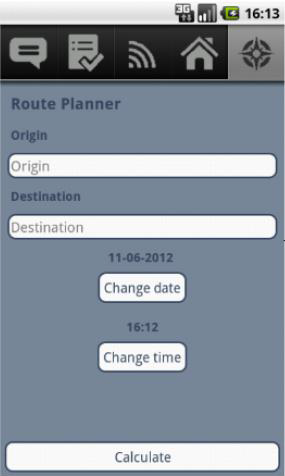
\includegraphics[width=1.5in]{current1.png}} \hspace{1em}%
\subfloat[\emph{Report information feature.}]{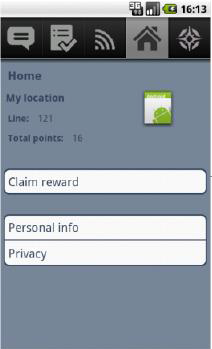
\includegraphics[width=1.5in]{current2.png}}
\subfloat[\emph{Trip information feature.}]{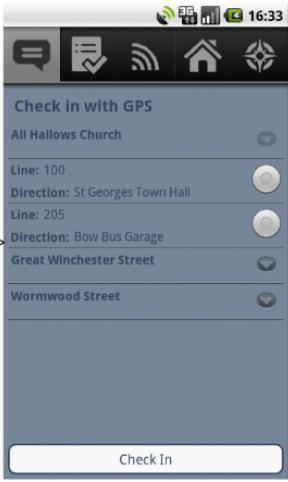
\includegraphics[width=1.5in]{current3.png}}
\caption{Screenshots of the previously implemented interface.}

\label{fig:current}
\end{center}
\end{figure}

\pagebreak

\section{User-Centered Design}

In the recent years, the attempt of several institutions to integrate design with technology has become a regular behaviour in the development of their products.
In 1999, it was established an international standard, \emph{ISO 13407}, that aimed to provide "guidance on achieving quality in use by incorporating user centred design activities throughout the life cycle of interactive computer-based systems."

That standard established four activities that had to be started at the earlier stages of a project:

\begin{itemize}
\item Understand and specify the context of use for the product - Collect relevant contextual information from the environment where the system is going to be used;
\item Specify the user and organisational requirements - Formulate and build the user-centered
requirements for the new software.
\item Produce design solutions - Simulate design solutions using paper or computer-based mockups and get feedback of real users;
\item Evaluate designs against requirements. Last but not least,is indispensable to evaluate
the design work performed previously. In this phase anomalies, defects, bugs, failures are detected in order to select the best solution for the system.
\end{itemize}

These activities were meant to be performed according to the following work flow.

\begin{figure}[h!]
  \begin{center}
    \leavevmode
    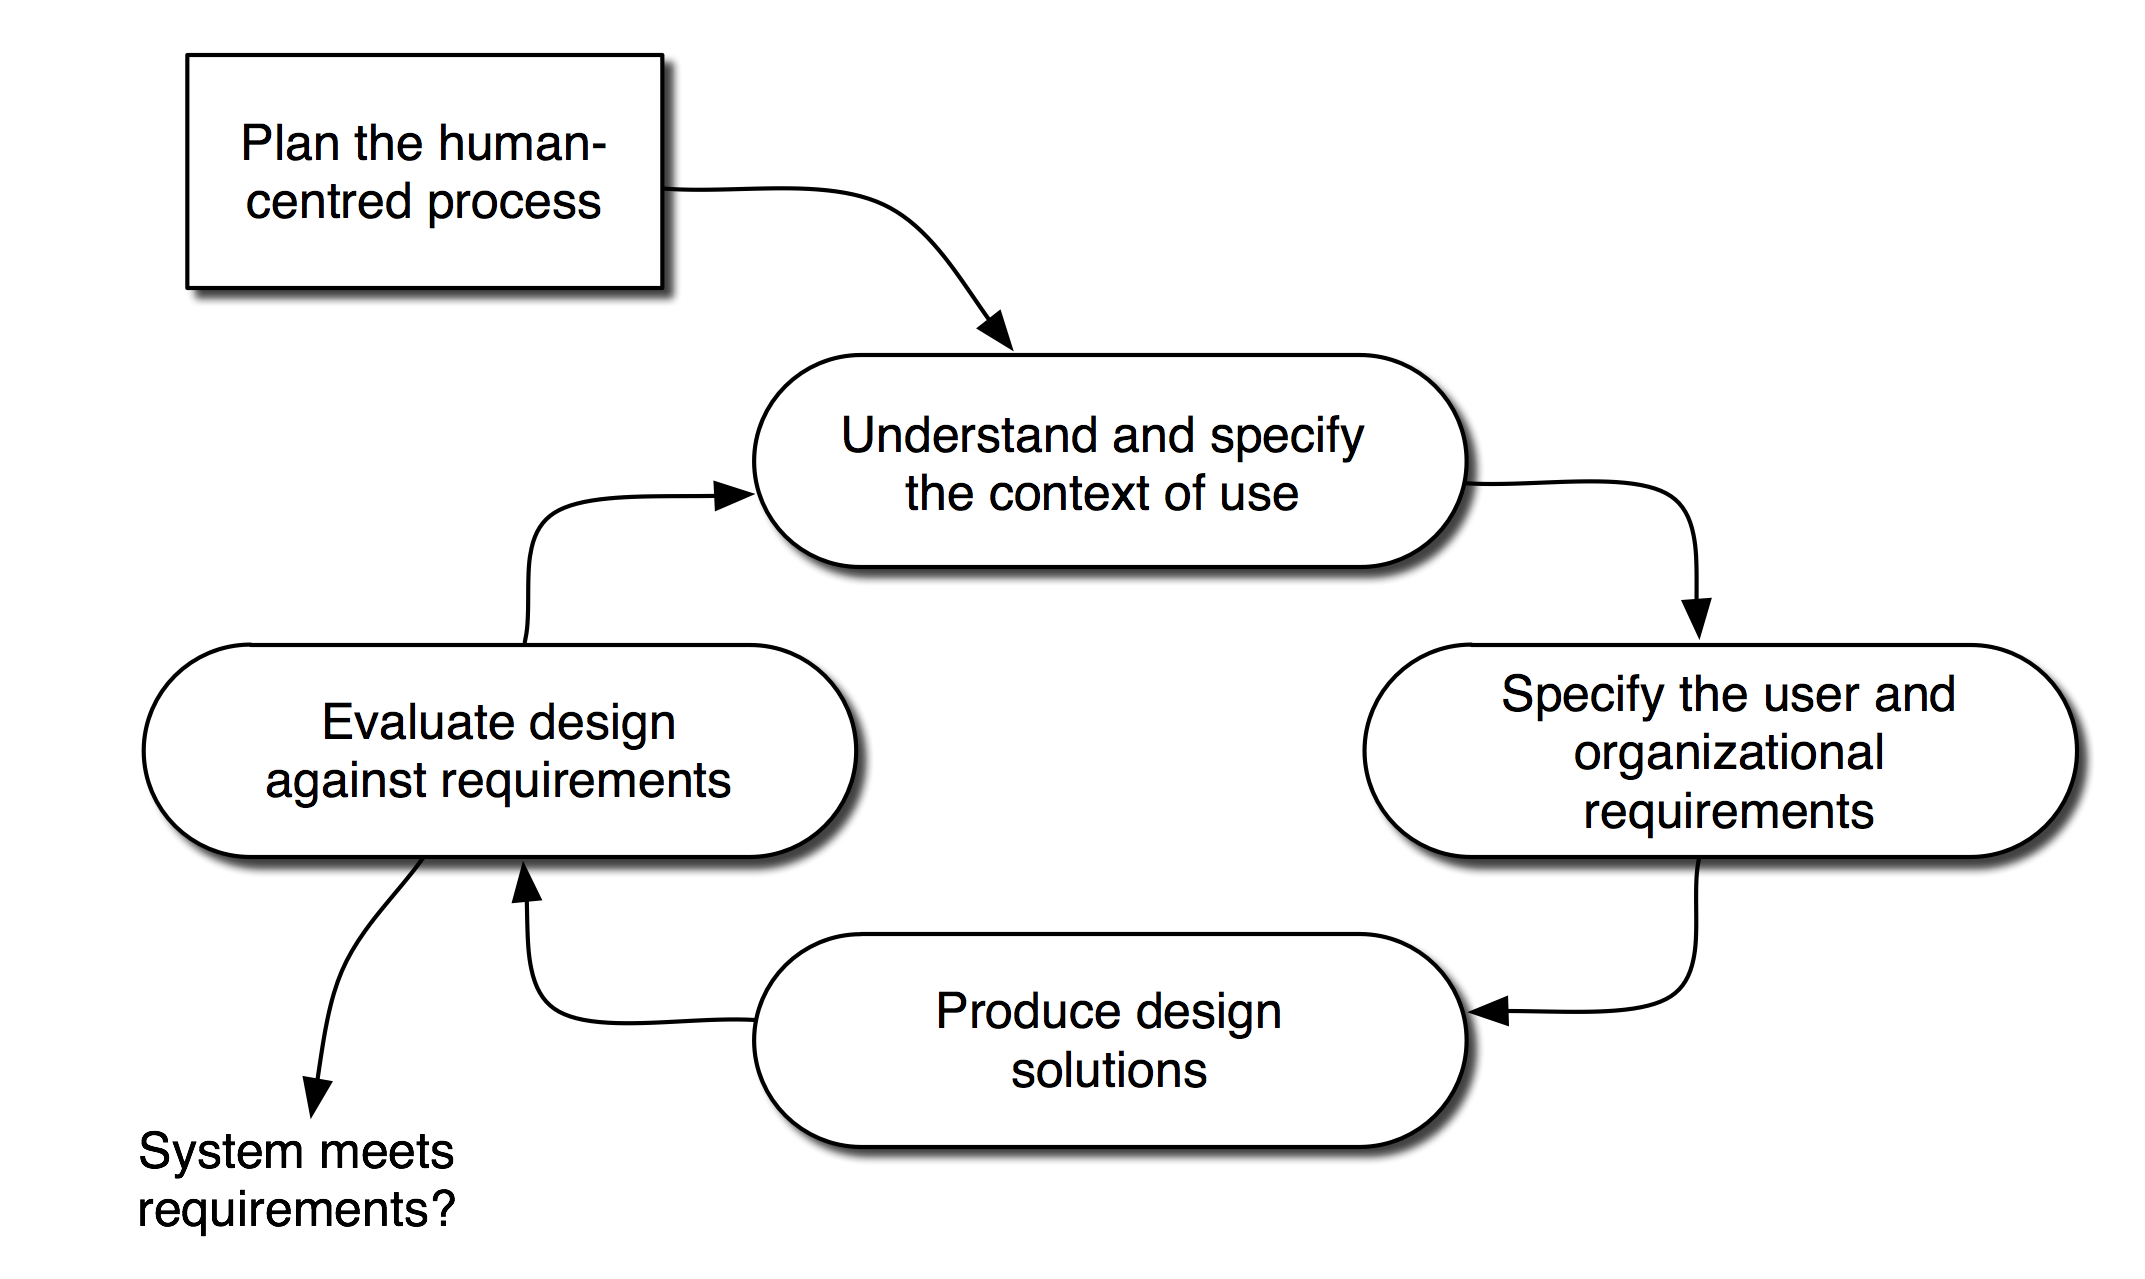
\includegraphics[scale=0.8]{iso13407.png}
    \caption{Workflow of the process described in ISO 13407.}
    \label{fig:iso}
  \end{center}
\end{figure}

This standard has since then been revised and re-issued as \emph{ISO 9241-210}, that describes six key principles to apply in a user-centered design process \cite{kn:Tra11}:

\begin{itemize}
\item The design is based upon an explicit understanding of users, tasks and environments. This means that is necessary to understand your users, understand what they want to do with the system and understand the environment in which the system is used.

\item Users are involved throughout design and development - Users must be involved in all design phases, not just at the start and at the end of the design.

\item The design is driven and refined by user-centred evaluation - Usability testing should be carried out throughout the design process. Initially, to test preliminary designs such as paper prototypes, and after that, not just at the end of the process.

\item The process is iterative - It is difficult, if not impossible, for users to explain what they want or need from a system. So, in order to find out what people want, it is necessary to show them something that they probably don't want (first designs) and then discover how to improve it. This means that if a waterfall methodology is used the design process will struggle to be user-centered.

\item The design addresses the whole user experience - Usability (and a good user experience) is about a lot more than making things simple, including the perceptual and emotional aspects typically associated with user experience.

\item The design team includes multidisciplinary skills and perspectives - The design team should include a range of views, including the voices of accessibility experts, end users, domain experts, etc.
\end{itemize}

Given those recommendations, the chosen process in order to achieve the expected results has four phases: 

\begin{itemize}
\item Requirements Elicitation phase;
\item Design phase - consists in the creation of alternative low-level designs, along with the usability tests and studies in order to maximize their quality and relevance.
\item Prototyping phase - Implementation of a chosen design, previously done, as an \emph{Android} mobile application.
\item Testing phase - Realization of usability tests.
\end{itemize}

This process is iterative, in order to involve potential users all along the design process and constantly improve the quality of the solution.

\section{Usability Evaluation}

The methods to perform the usability evaluation will encompass: 

\begin{itemize}
\item Surveys/questionnaires to potential users.
\item Usability tests perform in a laboratory environment.
\item Test with users in the field - The realization of a pilot test alongside potential users of the application on a real case scenario is one of the main goals to be achieved after the completion of the interface work.
\end{itemize}

\section{Usability Tests}

In the scope of this project, usability testing will be employed in order to test the acceptance of the final result along potential users, as well as comparing different versions of developed interfaces and identify the origin of possible unexpected/unwanted behaviours in its utilization.

Jakob Nielsen, one of the most known authors on the usability field, through deep experience in usability testing, has come up with a set of guidelines, checklists, methods and metrics that can be applied in those tests.

Between the set of metrics suggested by Nielsen, it is possible to find: 

\begin{itemize}
\item Success rate in accomplishing a task.
\item Number of clicks (or touches) needed to perform a task.
\item Error rate in accomplishing a task.
\item Severity of found errors.
\item Conclusion rate of a task.
\end{itemize}

However, the particular set of metrics to be chosen and tested in this project are not yet defined, and should be  defined in a posterior phase.






